\documentclass[aspectratio=169]{beamer}
\usepackage{lectureppt} % Load your custom style



\title{수리경제학}
\subtitle{미분 1: 도함수와 미분}
% \subtitle{직관적 이해와 활용 테스트트}
\author{이재석}
\date{2025-04-15}

\begin{document}

\begin{frame}
  \titlepage
\end{frame}

\begin{frame}{목차}
  \tableofcontents
\end{frame}

% \section{미분을} % 정의하는 방법 1 대수학 (Algebra)적 접근}
% \begin{frame}%{미분을 정의하는 방법 1: 대수학 (Algebra)적 접근}
%   \begin{itemize}
%     \item 함수 \( f(x) \)의 미분계수는 다음과 같이 정의됨
%     % \[ f'(x)=\lim_{h \to 0} \frac{f(x+h)-f(x)}{h} \]
%     \item 이 정의는 함수의 기울기를 나타내며, 접선의 기울기와 관련됨
%   \end{itemize}

% 제일 쉽고 간편하게 개념을 느끼고 사용하면 됨.
% 크게 세가지로 보여 줄 수 있음. 1. 대수학적으로 보여주기 2.기하학적적으로 보여주기 3.수학적 명제로 증명하기.
% 수학적 명제가 가장 완결성을 가지지만 추상적이기 때문에 '느끼기'힘듦.
% 대수학적으로 보여주고, 기하학적으로 보여주고, 다시 대수학적으로 살펴볼 것.
% 우리의 목적은 수하적으로 완결한 미분을 배우는것이 아니라, 아래 문제를 풀기 위함임.
% 1.효용극대화 2.이윤극대화 3.비용최소화
% 이 문제들은 미분을 통해 풀 수 있음.


\section{미분 홅아보기기}
\begin{frame}{미분의 정의와 의미}
  \begin{definition}[도함수]
    실수($\mathbb{R}$)의 어떤 함수 \textcolor{violet}{$f(x)$}가 정의되는 포인트 \textcolor{blue}{\emph{$a$}} 에서 \emph{미분가능(differentiable)} 하고, 정의역이 포인트 \textcolor{blue}{\emph{$a$}} 를 포함한다면, \textcolor{blue}{\emph{$a$}} 에서 \textcolor{red}{미분계수(순간변화율)} \textcolor{red}{\emph{$L$}} 은 \\
    \begin{equation}
      \textcolor{red}{L} = \textcolor{teal}{\lim_{h \to 0} \frac{f(\textcolor{blue}{a}+h)-f(\textcolor{blue}{a})}{h}}
    \end{equation}
  \end{definition}
  \begin{itemize}
    \item 미분하다: 함수 \textcolor{violet}{$f(x)$} 의 \textcolor{teal}{도함수}에 \textcolor{blue}{\emph{$x_0$}} 를 대입하여, \textcolor{red}{미분계수 $L$}의 값을 찾는다
    \item 어떤 함수 \textcolor{violet}{$f(x)$}를 미분하다 \\
    = \textcolor{violet}{$f(x)$} 의 \textcolor{red}{미분계수}를 구하다 \\
    = \textcolor{teal}{$f'(x \mid \textcolor{blue}{x = x_0})$}
    = \textcolor{teal}{$f'(x)$}를 구하다 \\
    = \textcolor{violet}{$f(x)$} 의 \textcolor{teal}{도함수}를 구하다 
    = \textcolor{teal}{$\frac{\mathbf{d}y}{\mathbf{d}x}$}
  \end{itemize}
\end{frame}


\begin{frame}{미분의 기하학(Geometry)적 접근  \( y = x \)}
  \begin{columns}
    \begin{column}{0.5\textwidth}
        \begin{itemize}
          \item 미분은 함수의 기울기를 나타내며, 기하학적으로는 접선의 기울기와 관련됨
          \item 함수의 그래프에서 특정 점에서의 접선의 기울기를 구하는 것이 미분의 본질
          \item 미분계수는 함수의 순간 변화율을 나타내며, 이는 접선의 기울기와 동일함
        \end{itemize}
    \end{column}
    \begin{column}{0.5\textwidth}
      % Add an image or diagram related to the geometric approach of differentiation
      % Example: A graph showing a function and its tangent line at a point
      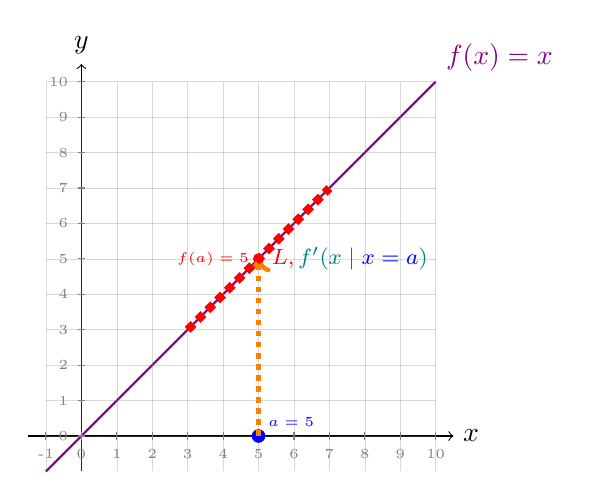
\begin{tikzpicture}[scale=0.45]
        % Draw axes
        \draw[->] (-1.5, 0) -- (10.5, 0) node[right] {\(x\)};
        \draw[->] (0, -1) -- (0, 10.5) node[above] {\(y\)};
  
        % Draw the line y = x in violet
        \draw[thick, violet, domain=-1:10] plot (\x, \x) node[above right] {\(f(x) = x\)};
  
        % Grid lines in gray
        \foreach \x in {-1,...,10}
          \draw[gray, very thin, opacity=0.3] (\x,-1) -- (\x,10);
        \foreach \y in {0,...,10}
          \draw[gray, very thin, opacity=0.3] (-1,\y) -- (10,\y);
  
        % Labels on axes in gray
        \foreach \x in {-1,0,...,10}
          \draw[gray] (\x,0.1) -- (\x,-0.1) node[below, gray] {\tiny \x};
        \foreach \y in {0,...,10}
          \draw[gray] (0.1,\y) -- (-0.1,\y) node[left, gray] {\tiny \y};
  
        % Blue dot at (5,0)
        \filldraw[blue] (5,0) circle (5pt) node[above right] {\tiny \(a = 5\)};
  
        % Red dot at (5, 5)
        \filldraw[red] (5,5) circle (4pt) node[left] {\tiny \(f(a) = 5\)};
  
        % Orange dotted arrow from (5,0) to (5,5)
        \draw[->, orange, line width=2pt, dotted] (5,0) -- (5,5);
  
        % Dotted red line from (3,3) to (7,7) with label
        \draw[red, dotted, line width=3pt] (3,3) -- (7,7) node[pos=0.5, right, red] {\footnotesize \(L, \textcolor{teal}{f'(x \mid \textcolor{blue}{x = a})} \)};
      \end{tikzpicture}
    \end{column}
    
  \end{columns}
\end{frame}


\begin{frame}{미분의 접근법: 기하학(Geometry) \( f(x) = x^2 \)}
  \begin{columns}
    \begin{column}{0.5\textwidth}
        \begin{itemize}
          \item 미분=함수의 기울기=접선의 기울기 \\
             미분은 접선의 기울기 <=> 접선의 기울기는 미분 \\
             미분계수는 함수의 순간 변화율=접선의 기울기
        \end{itemize}
    \end{column}
    \begin{column}{0.5\textwidth}
      % Add an image or diagram related to the geometric approach of differentiation
      % Example: A graph showing a function and its tangent line at a point
      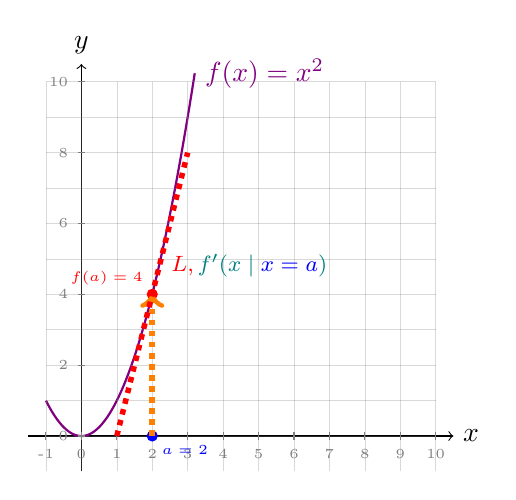
\begin{tikzpicture}[scale=0.45]
        % Draw axes
        \draw[->] (-1.5, 0) -- (10.5, 0) node[right] {\(x\)};
        \draw[->] (0, -1) -- (0, 10.5) node[above] {\(y\)};

        % Draw the function f(x) = x^2 in violet
        \draw[thick, violet, domain=-1:3.2, samples=100] plot (\x, {\x*\x}) node[right] {\(f(x) = x^2\)};

        % Grid lines in gray
        \foreach \x in {-1,...,10}
          \draw[gray, very thin, opacity=0.3] (\x,-1) -- (\x,10);
        \foreach \y in {0,...,10}
          \draw[gray, very thin, opacity=0.3] (-1,\y) -- (10,\y);

        % Labels on axes in gray
        \foreach \x in {-1,0,...,10}
          \draw[gray] (\x,0.1) -- (\x,-0.1) node[below, gray] {\tiny \x};
        \foreach \y in {0,2,...,10}
          \draw[gray] (0.1,\y) -- (-0.1,\y) node[left, gray] {\tiny \y};

        % Blue dot at (2, 0)
        \filldraw[blue] (2,0) circle (4pt) node[below right] {\tiny \(a = 2\)};

        % Red dot at (2, 4)
        \filldraw[red] (2,4) circle (4pt) node[above left] {\tiny \(f(a) = 4\)};

        % Orange dotted arrow from (2,0) to (2,4)
        \draw[->, orange, line width=2pt, dotted] (2,0) -- (2,4);

        % Tangent line: y = 4x - 4 (through (2,4), slope 4)
        \draw[red, dotted, thin, line width=2pt] (1, 0) -- (3, 8) 
          node[pos=0.6, right, red] {\footnotesize \(L, \textcolor{teal}{f'(x \mid \textcolor{blue}{x = a})} \)};
      \end{tikzpicture}
    \end{column}
    
  \end{columns}
\end{frame}


\begin{frame}{미분의 접근법: 기하학(Geometry) \( f(x) = x^2 \)}
  \begin{columns}
    \begin{column}{0.5\textwidth}
        \begin{itemize}
          \item 평균변화율: 구간 \( [a, b] \)에서 함수의 평균적 변화율 (delta y / delta x)
             \[ \frac{f(b)-f(a)}{b-a} \]
          \item 순간변화율: 특정 지점 \( x=a \)에서의 변화율 (미분계수) (dy / dx)
             \[ \lim_{h \to 0} \frac{f(a+h)-f(a)}{h} \]
        \end{itemize}
    \end{column}
    \begin{column}{0.5\textwidth}
      % Add an image or diagram related to the geometric approach of differentiation
      % Example: A graph showing a function and its tangent line at a point
      \begin{tikzpicture}[scale=0.45]
        % Draw axes
        \draw[->] (-1.5, 0) -- (10.5, 0) node[right] {\(x\)};
        \draw[->] (0, -1) -- (0, 10.5) node[above] {\(y\)};
      
        % Draw f(x) = 0.25 * x^2
        \draw[thick, violet, domain=0:6, samples=100] 
          plot (\x, {0.25*\x*\x}) 
          node[right] {\(f(x) = 0.25x^2\)};
      
        % Grid lines in gray
        \foreach \x in {-1,...,10}
          \draw[gray, very thin, opacity=0.3] (\x,-1) -- (\x,10);
        \foreach \y in {0,...,10}
          \draw[gray, very thin, opacity=0.3] (-1,\y) -- (10,\y);
      
        % Points a = 2 and b = 6
        \filldraw[blue] (2,1) circle (3pt) node[below left] {\tiny \(a=2\)};
        \filldraw[blue] (6,9) circle (3pt) node[above right] {\tiny \(b=6\)};
        \draw[thick, orange, dashed] (2,1) -- (6,9) 
          node[pos=0.5, above left, orange] {\small 평균 변화율: 2};
      
        % Point x = 2
        \filldraw[red] (4,4) circle (3pt) node[above left] {\tiny \(x = 2\)};
        \draw[->, orange, line width=1pt, dotted] (4,0) -- (4,4);
      
        % Tangent at x = 2: slope = 1, equation: y = x - 1
        \draw[red, dotted, very thick, domain=1:4] 
          plot (\x, {\x - 1}) 
          node[pos=0.9, above right, red] {\footnotesize \(L,\ f'(x) = 1\)};
      \end{tikzpicture}
      
    \end{column}
    
  \end{columns}
\end{frame}







\section{미분의 풀이법}
\begin{frame}{미분의 풀이법 : 기울기와 미분계수}
  \begin{itemize}
    \item askjdfkasdf
  \end{itemize}
\end{frame}

\begin{frame}{미분가능함의 의미}
  \begin{itemize}
    \item 함수 \( f(x) \)가 특정 점에서 미분가능하다는 것은 도함수가 그 점에서 존재함을 의미
    \item 함수가 부드럽고 연속적일 때 일반적으로 미분가능
  \end{itemize}
\end{frame}


\begin{frame}{미분의 풀이법 : 대수학적 접근 (Algebra)}
  \begin{itemize}
    \item askjdfkasdf
  \end{itemize}
\end{frame}



\begin{frame}{다항함수의 미분법}
  \begin{itemize}
    \item 1차 함수 \( f(x)=ax+b \), 도함수는 \( f'(x)=a \)
    \item 2차 함수 \( f(x)=ax^2+bx+c \), 도함수는 \( f'(x)=2ax+b \)
    \item 3차 함수 \( f(x)=ax^3+bx^2+cx+d \), 도함수는 \( f'(x)=3ax^2+2bx+c \)
  \end{itemize}
\end{frame}

\begin{frame}{implicite function}
  
\end{frame}



\section{미분이 필요한 함수형태}




\begin{frame}{생산함수와 MRTS}
  MRTS는 생산함수의 접선의 기울기.
  \begin{itemize}
    \item 콥더글라스 함수: \( f(x,y)=Ax^\alpha y^\beta \)
    \item 리니어 생산함수
    \item 레온티예프 함수: 완전 보완적 성질
  \end{itemize}
\end{frame}

\begin{frame}{콥더글라스 생산함수}
  
\end{frame}

\section{효용함수와 MRS}
\begin{frame}{효용함수}
  MRS는 효용함수의 접선의 기울기.
  \begin{itemize}
    \item 콥-더글라스 효용함수% (Cobb-Douglas Utility Function): U(x_1, x_2) = x_1^a * x_2^b
    \item 리니어 (완전 대체재) 효용함수% (Perfect Substitutes Utility Function): U(x_1, x_2) = ax_1 + bx_2
    \item 레온티에프 효용함수 %(Leontief% Utility Function): U(x_1, x_2) = min{ax_1, bx_2} (완전 보완재)
    \item 로그 효용함수 %(Log% Utility Function): U(x_1, x_2) = ln(x_1) + ln(x_2)
    \item 루트 효용함수 %(Square% Root Utility Function): U(x_1, x_2) = sqrt(x_1) * sqrt(x_2) 
  \end{itemize}
\end{frame}


\section{주요 미분 공식}

\begin{frame}{주요 미분 공식}
  \begin{itemize}
    \item Polynomial: \( (x^n)'=nx^{n-1} \)
    \item Fraction: \( \left(\frac{f(x)}{g(x)}\right)'=\frac{f'(x)g(x)-f(x)g'(x)}{g(x)^2} \)
    \item Exponential: \( (e^x)'=e^x \)
    \item Logarithmic: \( (\ln x)'=\frac{1}{x} \)
  \end{itemize}
\end{frame}

\begin{frame}{합성함수의 미분법}
  
\end{frame}

% \section{경제학에서 사용되는 함수와 미분법}

% \begin{frame}{경제학의 주요 함수와 미분법}
%   \begin{itemize}
%     \item 콥더글라스 함수: \( f(x,y)=Ax^\alpha y^\beta \), \(\frac{\partial f}{\partial x}=\alpha A x^{\alpha-1}y^\beta\)
%     \item Pseudo-linear 함수: 선형적 특성, 미분이 단순
%     \item 로그 함수: \( f(x)=\ln x \), \( f'(x)=\frac{1}{x} \)
%     \item 레온티예프 함수: 완전 보완적 성질, 특정 점에서만 미분가능
%   \end{itemize}
% \end{frame}


\begin{frame}{최적화 문제: 미분으로 해결}
  경제학의 두가지 문제
  \begin{itemize}
    \item 효용극대화\\
          argmax
    \item 이윤극대화\\
          argmax
    \item 비용최소화 (=이윤극대화)\\
          argmin
  \end{itemize}
  % \begin{itemize}
  %   \item 효용함수
  %   \item 최적소비조합
  %   \item 
  % \end{itemize}
\end{frame}







% \section{콥더글라스 함수와 미분}
% \section{콥더글라스 함수와 미분}
% \section{콥더글라스 함수와 미분}
% \section{콥더글라스 함수와 미분}


\section{음함수의 미분: 제약하의 최적}



\end{document}

